
One of the benefits of tag cloud visualisation is that data point textual identifiers (such as names) are a key part of the graphic, meaning that users don't have to navigate into the visualisation to find important information. With this in mind, the sort of data set that would be optimal to display in a tag cloud is one which includes textual information. Many datasets include this sort of information, in the form of names, labels or identifiers. In a general capacity, example datasets that might be used include brand names or marketing data, company financial information, stock market or foreign exchanges, country statistics (see Fig. \ref{fig:buglist}), animal endangerment ratings, sporting events, file and folder names in a computer, and so on. Software engineering datasets also contain this sort of data such as class, method or package names, bug categories and rankings (see Fig. \ref{fig:buglist}), and agile stories and tasks. 

\begin{figure}[h!]
	\centering
	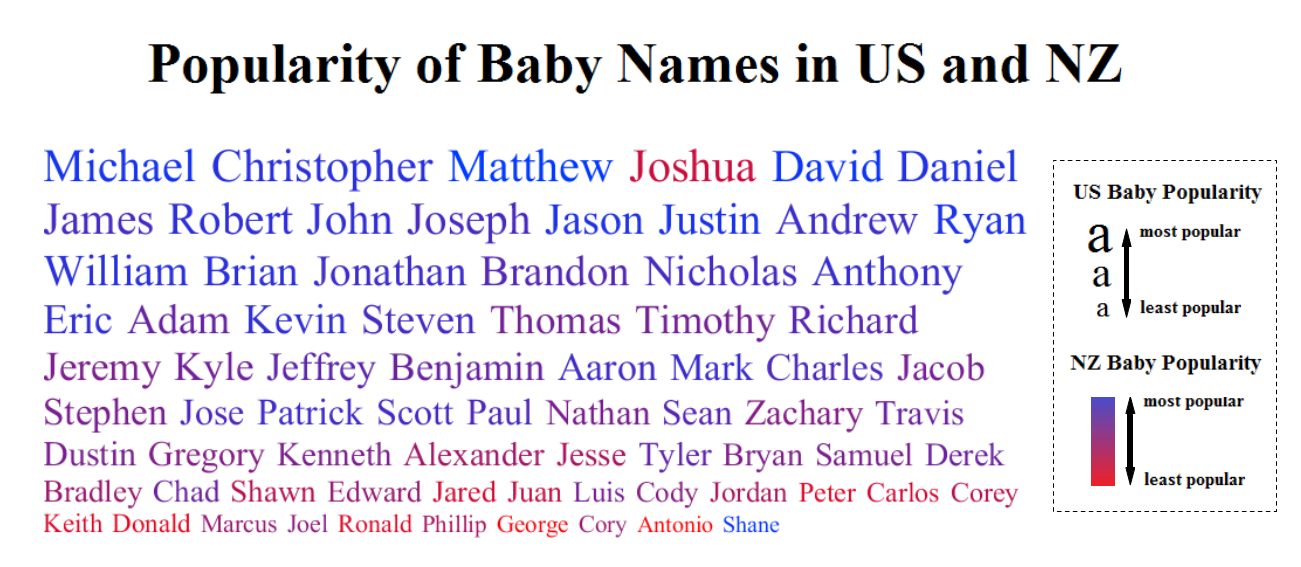
\includegraphics[scale=0.45]{babynames.png}
	\caption{\emph{Popularity of Baby Names}}
	\label{fig:babynames}
\end{figure}

\begin{figure}[h!]
	\centering
	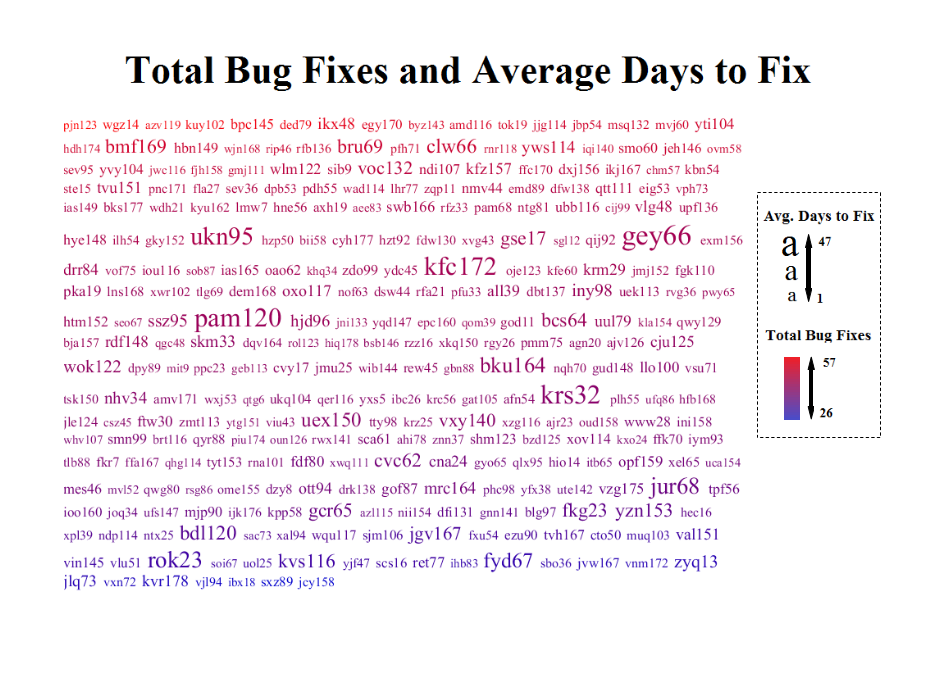
\includegraphics[scale=0.65]{buglist.png}
	\caption{\emph{Bug Fixes per User}}
	\label{fig:buglist}
\end{figure}

Much of the important textual data contained in these sorts of datasets is a phrase or collection of words rather than just one word. Also, many datasets containing some sort of label or identifier utilise many characters - such as a fully qualified file or class name. It is important to note that multiple word phrases and lengthy label names take up more real estate in the visualisation. There are two possible issues with this 1) it may have the effect of the data point appearing to have more importance than it actually does due to the increased prominence of the text and 2) with multiple word tags it may be difficult to distinguish the boundaries between data points. See Fig. \ref{fig:birds} for an example of these issues.

\begin{figure}[h!]
	\centering
	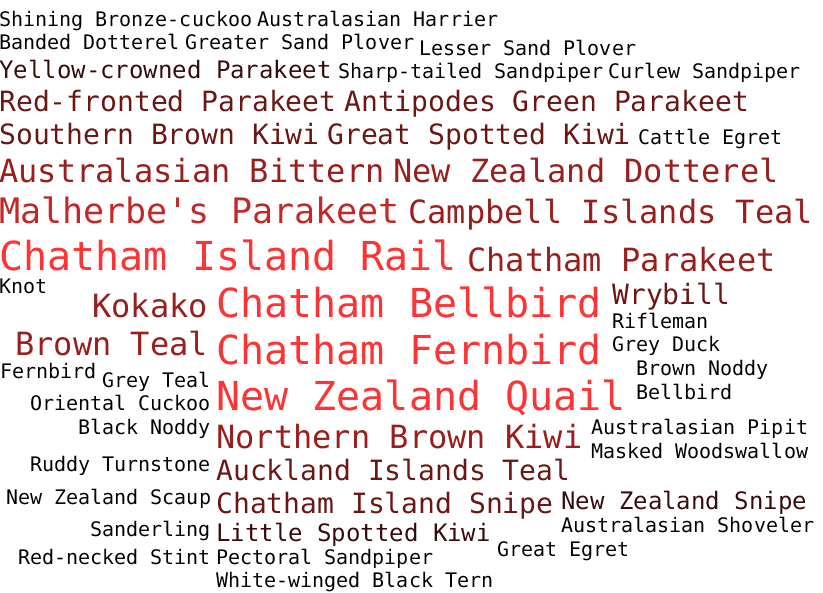
\includegraphics[scale=0.65]{birds.png}
	\caption{\emph{NZ Endangered Species Ranking - Birds}}
	\label{fig:birds}
\end{figure}




% ------------------------------------------------------------------------

%%% Local Variables: 
%%% mode: latex
%%% TeX-master: "../thesis"
%%% End: 
